\section{System Design}

Figure~\ref{fig:architect} shows the architecture of
Geo-Store~\cite{journals/internet/KuCWL}. The major components of
Geo-Store include a spatially-aware mapping module, an internal
indexing module~\cite{DBLP:journals/vldb/NeumannW10}, and a query
planner/analyzer module.

\begin{figure}
\centering
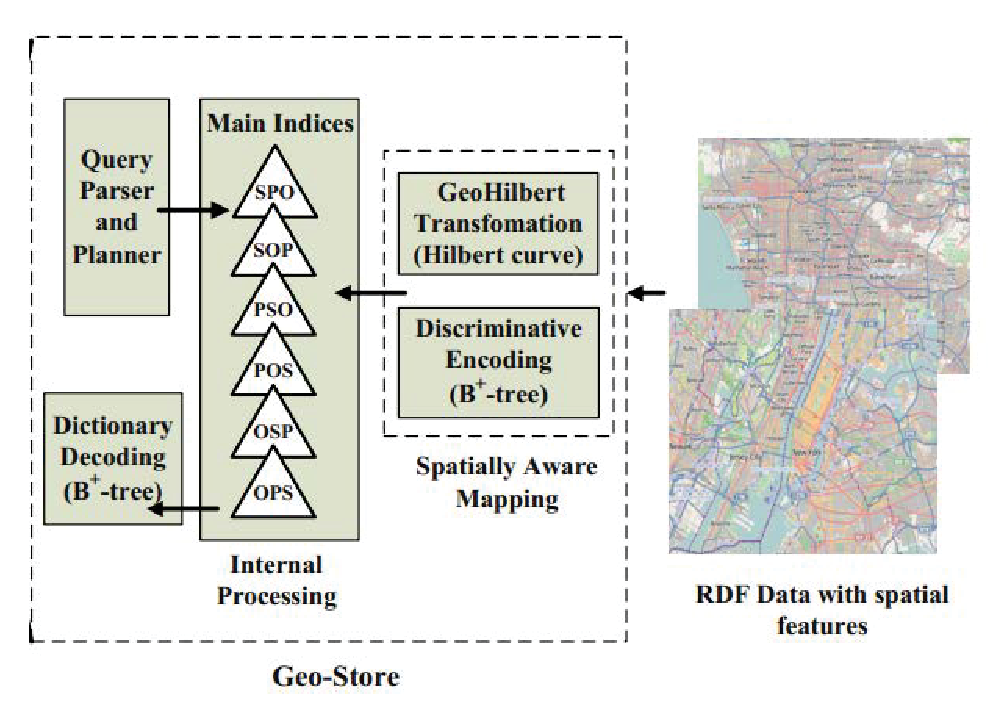
\includegraphics[width=3in]{images/architect.eps}
\caption{System Architecture of Geo-Store}\label{fig:architect}
\end{figure}

\subsection{The Spatially-Aware Hashing Module}

In order to support efficient spatial query processing, Geo-Store
employs Spatially-Aware Hashing (SAH), where Hilbert space filling
curves are generated and the Hilbert values (integers) of the
literals containing coordinates information (latitude/longitude)
are calculated and then appended to the original triple data
source as location indicators~\cite{journals/internet/KuCWL}.
Spatially-Aware Hashing provides the following advantages. First,
the Hilbert values of points of interest (POI) serves as
approximate location indicators. In other words, by only checking
with its Hilbert value, we can identify the small bounding grid (a
rectangular region) in which a specific POI resides. Second, those
location indicators perverse spatial locality, i.e., two POI's
that are geographically close are hashed into close integers at
most cases.  Third, the use of Hilbert values as location
indicators bases spatial query processing on integer number
comparison, reducing the occurrence of long string
(latitude/longitude) comparison, which is very costly in
computation and storage in triple stores.


\subsection{Spatial Query Analyzer}

In Geo-Store, spatial queries are expressed by using spatial query
filters and those filter are processed by our query analyzer.
When a query is submitted, the query analyzer looks for any
spatial filter in that query. If there is any spatial filter, the
analyzer uses the spatial-aware hashing to identify a list of
Hilbert values (serve as integer location indicators) that are
involved by the filter. Since the underlying triple store,
RDF-3X~\cite{DBLP:journals/vldb/NeumannW10}, are built on standard
SPARQL patterns without awareness of any spatial context, our
query analyzer then translates the related hash values into query
patterns and insert them as the patterns into the original query.
For multiple spatial query filters, the query analyzer applies
intersection operations to find the geographic locations
satisfying all the spatial constraints.
